\chapter{Wireless Security}

\section{Einleitung}

\section{Vorbereitungen}

Voraussetzungen für die weiteren Übungen:\\

- Alfa USB WLAN-Adapter\\
- Workstation/Notebook\\
- Virtual Box mit Kali Linux Image (+ Extension Pack)\\
- Grundlegende Kenntnisse mit Linux\\

Konfiguration des Alfa Adapters in Kombination mit Virtual Box:\\

Anschluss des Adapters über das beigelegte Y-Kabel an den Host.
In Virtual Box die Kali Maschine auswählen $\rightarrow$ Rechtsklick: Ändern $\rightarrow$ USB auswählen $\rightarrow$ USB-2.0-Controller aktivieren $\rightarrow$ USB-Filter hinzufügen
$\rightarrow$ Ralink WLAN auswählen (falls nicht vorhanden im GeräteManager nach dem WLAN Adapter suchen) $\rightarrow$ Mit OK bestätigen.\\
%Zusätzlich einen neuen Filter anlegen und Hersteller- bzw. Produkt-ID aus dem ersten Filter übernehmen. Die anderen Felder können unausgefüllt werden
Den WLAN Adapter ausstecken\\

Kali Linux in Virtual Box starten (user: root, passwort: toor)\\
Sobald die VM hochgefahren ist, den Adapter einstecken.\\
USB Icon im Fenster der Maschine sollte rot/grün blinken.\\ %(evtl screenshot)\\

\section{WEP}

\section{WPA/WPA2}
%Teilweise aus:
%http://www.elektronik-kompendium.de/sites/raspberry-pi/2008101.htm

WPA bzw. WPA2 (WiFi Protected Access) ist eine Kombination aus Authentifizierung und Verschlüsselung, um ein WLAN sicher zu betreiben. Die Authentifizierung erfolgt in der Regel mit einem Passwort, um den Zugriff durch unberechtigte Personen zu verhindern. Möchte ein Angreifer nun in das Netzwerk eindringen, muss er dieses Passwort herausfinden.\\


Grundsätzlich gibt es beim Hacken keine Unterschiede zwischen WPA- und WPA2-gesicherte WLANs. Die Authentifizierungsmethode ist im Prinzip identisch. Der Unterschied liegt im Verschlüsselungsverfahren, welche für die typischen Hacking-Methoden auf WPA-gesicherte WLANs nicht relevant ist.\\ Grund dafür ist, dass WPA2 derzeitig noch als nicht zu knackendes Verschlüsselungsverfahren
gilt und daher ein Angriff auf die Verschlüsselung vergebene Mühe wäre. \\

Der typische Angriff gegen ein WPA-/WPA2-gesichertes WLAN läuft über reines Bruteforcing oder einer sogenannten Wörterbuch-Attacke (engl. dictionary-attack). Bei ersterem werden einfach alle Kombinationen bestehend aus Buchstaben, Ziffern und Sonderzeichen, oder nur einem Ausschnitt davon, bis zur gewünschten Länge getestet. Je nach Länge und Komplexität des Passworts kann sich dieser Vorgang über viele Stunden, bis zu Tagen und sogar mehreren Jahren hinziehen. Häufig wird bei einer Bruteforce-Attacke zuvor eine Wordlist, wie bei einem Dictionary-Angriff, mit allen zu testenden Kombinationen erstellt. Bei einem Wörterbuch-Angriff wird somit durch die Passwortkandidaten in einer riesigen Wordlist iteriert und mit dem herauszufindenden Passwort abgeglichen. %wie abgeglichen? verhasht ,bzw. verschlüsselt? 
Stimmen beide überein, wurde das Passwort gefunden. Diese Wörterlisten können entweder selber generiert werden oder sind auch im Internet zu finden. Wie wir später noch sehen werden, gibt es auch hybride Ansätze, die beide Angriffsarten verknüpfen.\\


Ein WPA-Handshake findet zwischen Access Point und WLAN-Client statt, wenn der WLAN-Client sich mit dem WLAN verbinden will. Dieser WPA-Handshake muss aufgezeichnet werden. Anschließend wird bei einem Wörterbuch-Angriff mit Hilfe der Wordlist das WLAN-Passwort erraten. Ein erfolgreicher Angriff steht und fällt mit einer guten Wordlist, in der das WLAN-Passwort enthalten sein muss. Darin besteht die eigentliche Schwierigkeit bei einem WPA/WPA2-WLAN-Hack.\\


Grober Ablauf eines WPA-/WPA2-Hacks:

\begin{enumerate}
\item Wordlist erstellen oder besorgen 
\item Grundzustand herstellen und Monitor Mode einschalten
\item WLAN mit WPA/WPA2 identifizieren (Information Gathering) 
\item Datenverkehr mit Airodump-ng aufzeichnen
\item Deauthentication-Attacke mit Aireplay-ng (optional)
\item WPA-Passwort mit Hilfe der Wordlist herausfinden
\end{enumerate}

%more space

\textbf{\Large{Cracking des WPA Keys}}\\ %(evtl mit Screenshots oder weiter ausformulieren)

{\Large 1. Check des WLAN Adapter}\\

Zuerst muss geprüft werden, ob der eingesteckte USB WLAN-Adapter erkannt wird und somit einsatzbereit ist. Dazu das Terminal öffnen in Kali Linux öffnen und folgenden Befehl eingeben. 

$$iwconfig$$\\

Der Adapter sollte als Interface, meist WLAN0 oder WLAN1, angezeigt werden\\
Im Folgenden muss bei allen Befehlen die Interface Bezeichnung mit der hier angezeigten ersetzt werden, da sie sich von Rechner zu Rechner unterscheiden kann.\\


{\Large 2. MAC-Spoofing}\\

Im Sinne von Wireless Security sollte man sich immer im Klaren sein, dass ein Angreifer immer in der Lage ist seine MAC-Adresse zu verändern. Dieser Vorgang wird auch Spoofing genannt.

Die MAC-Adresse ist eine herstellerspezifische Kennung, die fest einem Netzwerkgerät zugeordnet ist. Jede Adresse ist eindeutig. Findet man die MAC-Adresse eines Angreifers heraus, kann mit Hilfe dieser Identifikationskennung festgestellt werden, welchen Typ von Antenne er verwendet. Diese Erkenntnis kann helfen einen Angreifer zu identifizieren.
Verwendet ein Angreifer nun eine gefälschte MAC-Adresse können keine Rückschlüsse auf seine Identität gezogen werden, da überall nur seine Fake-Adresse angezeigt wird.\\

Zuerst muss dafür das WLAN Interface deaktiviert werden. Danach kann mit dem Kommando \textit{macchanger} die Adresse geändert werden.\\

\begin{equation*}
\begin{split}
ifconfig~wlanX~down\\
macchanger~\text{-}r~wlanX
\end{split}
\end{equation*}

\textit{X = NUM für das interface}\\

Beim Bestätigen des Befehls mit Enter, wird die eigene MAC-Adresse in eine zufällige generierte MAC-Adresse geändert und auf der Konsole angezeigt. Anschließend kann das Interface mit folgendem Befehl wieder aktiv gesetzt werden.\\
 
$$ifconfig~wlanX~up$$

\textit{X = NUM für das interface}\\


Mit dem Befehl\\ 
$$ifconfig~wlanX$$

\textit{X = NUM für das interface}\\

kann überprüft werden, ob die gespoofte MAC-Adresse auch aktiv ist.\\

{\Large 3. Das Interface in den Monitor Mode versetzen}\\

Damit mit dem WLAN Adapter Pakete aufgezeichnet werden können, muss sich der Adapter im Monitor Mode, oder auch Packet Injection Mode genannt, befinden. Dies wird mit folgendem Befehl erreicht.

$$airmon\text{-}ng~start~wlanX~$$

\textit{X = your number from iwconfig}\\

Mit dem Befehl\\ 

$$airmon\text{-}ng~check~kill$$

\textit{X = NUM für das interface}\\


werden alle andere Prozesse beendet, die auch auf den Netzwerkadapter zugreifen können. So können Konflikte beim Zugriff auf die Ressource vermieden werden.\\

{\Large 4. Aufzeichnen der WLAN Pakete mit airodump}\\
	
Im nächsten Schritt werden die WLAN Pakete aus der Umgebung aufgezeichnet. Damit möchte man einen Handshake zwischen dem zu hackenden Access Point und einem Client aufzeichnen. Anhand dessen kann anschließend das Passwort herausgefunden werden.\\

Mit dem folgenden Befehl können wir in den Aufzeichnungsmodus umschalten.
	
	$$airodump\text{-}ng~\text{-}b~a~wlanXmon$$\\
	 
	\textit{X = NUM für das interface}\\
	\textit{-b a = Scan im 5GHz Band}\\	
	
Falls wir im im 5GHz Bereich scannen möchten muss der Parameter \textit{-b a} mitgegeben werden. Falls nicht, kann der Parameter einfach weggelassen werden.\\	
Sollten keine Daten aufgezeichnet werden, dann den Adapter mehrmals aus- und wieder einstecken. 
Nach einem Reconnect muss der Adapter natürlich wieder in den Monitoring Modus versetzt werden.
	
Hat alles soweit geklappt, sollten alle erreichbaren SSIDS mit ihren jeweiligen Sendern angezeigt werden.\\ 
	
Als nächstes sollte die MAC-Adresse und der verwendete Kanal des zu hackenden APs notiert.
Anschließend kann durch einen neuen airodump-ng Durchlauf mit der MAC und dem Kanal als Parameter (nähere Infos unter \(man~airodump-ng\) abrufbar) der Scan
	eingeschränkt werden. Zusätzlich kann auch der Name der Ausgabedatei festgelegt werden. 
Der Befehl sieht dann in etwa wie nachfolgend aus.
	$$airodump\text{-}ng~\text{-}c~Kanal~\text{-}b~a~\text{-}\text{-}bssid~MAC\text{-}AP~\text{-}showack~\text{-}w~Filename~wlanXmon$$
	
		\textit{X = NUM für das interface}\\
		\textit{Kanal = der Kanal auf dem gelauscht werden soll}\\
		\textit{MAC-AP = die MAC-Adresse des Access Points}\\
		\textit{Filename = in die zu schreibende Datei}\\

	Verbindet sich nun ein Client auf den AP, so kann der 4-way-handshake mitgelesen werden, was auch in der Konsole, in der rechten oberen Ecke, angezeigt wird.
	Hat dies funktioniert, ist der erste Schritt für das Hacken des Passworts abgeschlossen.\\

{\Large 5. Cracken des Passworts}\\
		
Ab hier werden verschieden Tools und Angriffsarten für das Cracken des Keys vorgestellt.\\	

 \textbf{Dictionary Attack mit aircrack}\\

Dazu wird ein Dictionary File mit allen Passwörtern benötigt, die auf Übereinstimmung mit dem PSK gecheckt werden sollen. Auf dem Image sollt bereits eine Dictionary Datei im Home Verzeichnis vorhanden sein.

Mit folgendem Befehl kann der Dictionary-Angriff gestartet werden. 

$$aircrack\text{-}ng~\text{-}w~dict.file~\text{-}b~MAC\text{-}AP~File.cap$$

\textit{dict.file = Pfad zu dem Dictionary}\\ 
\textit{MAC-AP = Die MAC-Adresse des APs}\\ 
\textit{File.cap = Pfad zu dem cap file}\\

\textbf{Brutefore Angriff mit aircrack und crunch}

\begin{equation*}
\begin{split}
crunch~8~12~abcdefghijklmnopqrstuvwxyzABCDEFGHIJKLMNOPQRSTUVWXYZ \\
|~aircrack\text{-}ng~\text{-}\text{-}bssid~00:11:22:33:44:55~\text{-}w\text{-}~hack\text{-}wifi\text{-}01.cap
\end{split}
\end{equation*}
 
\textit{8 12 = die zu testende Passwortlängen, hier von Länge 8 bis 12}\\
\textit{abcde.. = die zu testenden Zeichen}\\



\textbf{Attacken mit hashcat}\\

Bei hashcat handelt es sich wohl um den derzeit schnellsten Passwortcracker auf dem Markt. Wir verwenden es als Alternative zu crunch.\\

Convert the .cap file in a hccap file\\

$$aircrack\text{-}ng~Filename.cap~\text{-}J~newFilename$$

\textit{Filename.cap = Pfad bzw. Name des alten .cap files}\\
\textit{Pfad bzw. Name des neuen .hccap file}\\

%+ Brutefore/Dictionary/Rule-Based Attack with hashcat möglich

Mit hashcat --help kann eine Hilfeseite aufgerufen werden in welcher der Befehl, die Parameter und die Verwendung
genauer erläutert werden. Falls Probleme auftreten oder detailliertere Einstellungen vorgenommen werden sollen, kann 
die Hilfeseite die erste Anlaufstelle sein.\\

\textbf{Dictionary Attack mit hashcat}

$$hashcat~\text{-}m~2500~capture.hccap~dict.txt$$\\

\textit{-m 2500 = Anweisung, dass ein WPA/WPA2 Key gecrackt werden soll}\\
\textit{caputre.cap = Pfad bzw. Name des hccap file}\\
\textit{dict.txt = Pfad bzw. Name des dictionary file}\\

Anschließend nutzt hashcat das Dictionary um das Passwort zu finden.
Mit Enter kann der aktuelle Status des Vorgangs abgefragt werden.\\ 

\textbf{Bruteforce Attack mit hashcat}

$$hashcat~\text{-}m~2500~\text{-}a3~capture.hccap~?d?d?d?d?d?d?d?d~(?d = 0\text{-}9)$$

\textit{-m 2500 = Anweisung, dass ein WPA/WPA2 Key gecrackt werden soll}\\
\textit{-a3 = Verwende Bruteforce}
\textit{caputre.cap = Pfad bzw. Name des hccap file}\\
\textit{?d..?d = definierte Maske für zu testenden Passwortkandidaten, Anzahl entspricht "bis zu Länge"\\
Weitere Optionen:\\
?l = abcdefghi...yz\\
?u = ABCDEFGHI...YZ\\
?s = Sonderzeichen\\
?a = ?l?u?s?d}\\

Bei der Bruteforce Attacke werden alle Kombinationen von Buchstaben bis zu einer bestimmten Länge durchgetestet.
Als letzter Parameter kann eine Art Maske angegeben werden, mit welcher die Länge und die zu testenden Ziffern, Buchstaben
und Zeichen festgelegt werden. Im Beispiel werden alle bis zu neunstelligen Zahlenkombinationen von hashcat durchprobiert.\\ 

\textbf{rule-based Attack mit hashcat}

$$hashcat~\text{-}m~2500~\text{-}r~/usr/share/hashcat/rules/best64.rule~capture.hccap~ dict.txt$$\\

\textit{-m 2500 = Anweisung, dass ein WPA/WPA2 Key gecrackt werden soll}\\
\textit{-r Pfad zum rules file = Verwende rule-based Angriff und Pfad}\\

rule-based attacks gehören zu den komplizierteren Angriffsarten. Dabei wird ein nomaler Dictionary-Angriff gefahren, aber mit rules erweitert. 
Die rules, zu deutsch Regeln, sind wie eine Art Programmiersprache
für die Generierung von Passwörtern. Es gibt Funktionen mit denen Passwortkandidaten bearbeitet, mit anderen Wörtern verknüpft oder bestimmte Kombinationen 
übersprungen werden können. Regeln zu schreiben kann sehr aufwendig sein und erfordert viel Wissen über Passwörter. Daher kann für die ersten Versuche auch 
die best64.rule Regel verwendet werden, die standardmäßig bei hashcat dabei ist.\\


%DoS Attack mit MDK3

%Erst den Adapter wieder in den Monitoring Mode versetzen.

%airmon-ng start wlanX

%disconnect bei verwendung von mdk3

\textbf{Cracking des Passworts mit Hilfe der Grafikkarte}\\

Neben dem normalen Hashcat gibt es eine weitere Version, die sich oclHashcat nennt. Mit dieser Version ist es möglich das Cracken Keys mit Hilfe der Grafikkarte durchzuführen. Hierfür sind die Geschwindigkeiten stark von der Leistungsfähigkeit der verwendeten Grafikkarten abhängig. 
Jedoch sind deutliche Leistungssteigerungen gegenüber der CPU in den meisten Fällen, bei halbwegs aktueller Hardware, zu erwarten. Notwendig sind aktuelle Treiber, die auf dem System installiert sein müssen. Weitere Infos dazu gibt es auf der Homepage von oclHashcat. 
Weiter ist es möglich mehrere Grafikkarten im Clusterbetrieb parallel für das Cracken eines Keys zu betreiben. Dadurch können noch größere Performancesteigerungen erzielt werden.

Leider ist es nicht möglich oclHashcat aus der virtuellen Maschine heraus zu verwenden, da der direkte Zugriff auf die Grafikkarte verweigert wird. Das Cracken per GPU kann hier deshalb nur exemplarisch beschrieben werden. Natürlich steht es jedem frei, mit dem hier gezeigten Verfahren auch zu Hause auf seinem privaten Rechner zu experimentieren.\\

\textit{Anwendungsfall}\\

Als Anwendungsfall wollen wir die Standard WLAN Keys von den Herstellern untersuchen. Oft werden von diesen längere Zahlenketten als default gesetzt. Natürlich könnte der Vergleich von CPU zu GPU auch mit anderen Passwörtern durchgeführt werden. 

In unserem Beispiel (FritzBox) ist vom Hersteller aus eine 16-stellige Ziffernfolge als Key gesetzt. Das Wissen, dass es sich nur um Ziffern handelt kann später beim Cracken ein deutlicher Vorteil sein.

Zuerst wird, wie in den oberen Kapiteln der Handshake zwischen dem Access Point und einem Client aufgezeichnet. Anschließend muss das aufgezeichnete .cap File für hashcat wieder in ein .hccap File umgewandelt werden. Wie dies funktioniert ist in den vorherigen Kapiteln bereits beschrieben worden. \\

Im nächsten Schritt soll einmal mit der CPU und einmal mit der GPU der Key herausgefunden werden. Dazu wird hashcat für den Durchlauf auf dem Prozessor und einmal oclHashcat, eine spezielle Version für die GPU, verwendet.\\ 

\textit{Durchführung 1}\\

Der erste Versuch wird wieder mit hashcat ausgeführt. Dazu wird der Befehl wie in dem vorhergehenden Kapiteln verwendet. Wir wissen nun aber, dass der Schlüssel eine Länge von 16 Zeichen besitzt und wir somit die Längen 1 - 15 nicht testen müssen. Dazu wird der Befehl um einen weiteren Parameter, der die einzige zu testende Länge angibt, erweitert.
%stimmt der befehl so??
$$hashcat~\text{-}m~2500~\text{-}a3~capture.hccap~\text{-}\text{-}pwd\text{-}min\text{=}16~?d?d?d?d?d?d?d?d~(?d = 0\text{-}9)$$\\

\textit{-m 2500 = Anweisung, dass ein WPA/WPA2 Key gecrackt werden soll}\\
\textit{-a3 = Verwende Bruteforce}
\textit{caputre.cap = Pfad bzw. Name des hccap file}\\
\textit{?d..?d = definierte Maske für zu testenden Passwortkandidaten, Anzahl entspricht "bis zu Länge"\\}\\


Die folgende Abbildung zeigt die Ausgabe sobald mit Enter der Befehl bestätigt wurde.\\

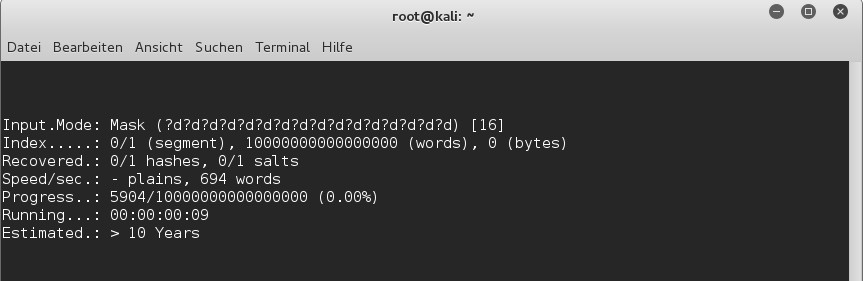
\includegraphics[width=\textwidth]{bilder/wlan/wlan_screenshot_1.png}\\

Dort sind einige interessante Informationen zu dem Durchlauf zu sehen. Die Geschwindigkeit beträgt knapp 700 Wörter pro Sekunde und dürfte sich für die meisten Prozessoren in diesem Bereich bewegen.
Als wichtigste Info wird die geschätzte Zeit für das Cracken betrachtet. Man sieht, dass hier mehr als 10 Jahre angenommen werden. Dies ist auch nicht weiter verwunderlich, wenn man den Blick auf die riesige Anzahl an Kombinationsmöglichkeiten richtet. Selbst durch die genaue Länge und dem Wissen, dass es sich nur um Zahlenkombinationen handelt konnte die Laufzeit nicht auf ein erträgliches Maß gesenkt werden. Somit ist das Cracken des Keys nicht mit einem einzelnen Prozessor und wohl auch nicht mit einer kleinen Anzahl an Rechenwerken möglich.\\

\textit{Durchführung 2}\\

Dieselbe Berechnung soll nun auf der Grafikkarte durchgeführt werden. Dazu wird oclHashcat verwendet, welches kostenfrei von deren Website heruntergeladen werden kann. Das Tool wird einfach entpackt und je nach Betriebssystem über die Kommandozeile gestartet. Der Befehl auf einem Windows System sieht folgendermaßen aus und ähnelt sehr stark dem vorherigen Aufruf.

$$cudaHashcat64.exe~\text{-}m~2500~\text{-}a~3~capture.hccap~\text{-}pwd\text{-}min\text{=}16~?d?d?d?d?d?d?d?d~(?d = 0\text{-}9)$$

\textit{-m 2500 = Anweisung, dass ein WPA/WPA2 Key gecrackt werden soll}\\
\textit{-a 3 = Verwende Bruteforce}
\textit{caputre.cap = Pfad bzw. Name des hccap file}\\
\textit{?d..?d = definierte Maske für zu testenden Passwortkandidaten, Anzahl entspricht "bis zu Länge"\\}\\

Wurde der Befehl bestätigt, kann mit der Taste "s" der Status des Vorgangs eingesehen werden. Einige Dinge sind bereits aus dem vorherigen Aufruf bekannt. Interessant sind die Keys per second, die getestet werden. Der Wert liegt hier bei 41586. Somit liegt der Speedup im Vergleich zur CPU bei fast 60facher
Geschwindigkeit. Dies ist natürlich deutlich schneller als im vorherigen Durchlauf. Jedoch wird auch in diesem Fall eine geschätzte Zeit von über 10 Jahren angezeigt. Das bedeutet, dass trotz der besseren Performance keine signifikante Verringerung der Laufzeit erreicht wurde. 
Letztendlich kann nun auch mit einer einzelnen GPU dieser Standard Key nicht geknackt werden.\\

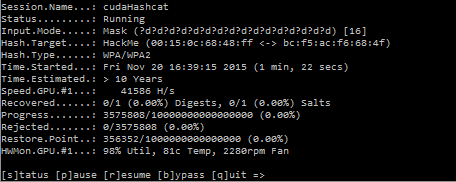
\includegraphics[width=\textwidth]{bilder/wlan/cudaHashcatNUMSeriesCrack.png}\\

%evtl noch Diagramm hier


\section{WPS}

\section{Sicherungsmaßnahmen}


